\documentclass{beamer}
%
% Choose how your presentation looks.
%
% For more themes, color themes and font themes, see:
% http://deic.uab.es/~iblanes/beamer_gallery/index_by_theme.html
%
\mode<presentation>
{
  \usetheme{default}      % or try Darmstadt, Madrid, Warsaw, ...
  \usecolortheme{default} % or try albatross, beaver, crane, ...
  \usefonttheme{default}  % or try serif, structurebold, ...
  \setbeamertemplate{navigation symbols}{}
  \setbeamertemplate{caption}[numbered]
} 

\usepackage[spanish]{babel}
\usepackage[utf8x]{inputenc}

\title[Clase 5]{Procesamiento de bases de datos con STATA}
\subtitle{Clase 5}
\author{Claudia Vazquez}
\date[]{\texttt{clauvazqu@gmail.com}\\Centro REDES}
\pgfdeclareimage[height=0.5cm]{university-logo}{logo-redes}
\logo{\pgfuseimage{university-logo}}

\begin{document}

\begin{frame}
  \titlepage
\end{frame}

\begin{frame}{Contenido}
  \tableofcontents
 \end{frame}

\begin{frame}{Introducción}
\begin{itemize}
\item Los gráficos son una excelente manera de comunicar información cuantitativa.
\item Son más fáciles de interpretar que las tablas cuando estamos dando una presentación.
\item Se recomienda no ``decorar'' excesivamente los gráficos (mantener el diseño lo más sencillo posible). 
\item \underline{Siempre} usar etiquetas para referenciar los ejes.
\item Veremos un pantallazo general pero no agotaremos todas las posibilidades que tiene el programa. Puede ver más en:  \url{http://www.stata.com/support/faqs/graphics/gph/stata-graphs/}
\end{itemize}
\end{frame}
\section{histograma}

\begin{frame}{Histograma}
\begin{itemize}
\item El histograma es una de las maneras más simples de representar una distribución. 
\item Se divide el soporte en intervalos iguales y en el eje vertical se grafica la proporción de obsrvaciones que cae dentro de cada intervalo (frecuencia relativa).
\item La sintaxis es simple: \texttt{histogram \textit{varname}}. 
\item Luego (después de una coma) pueden agregarse opciones como:
\begin{itemize}
\item \texttt{bin()}: modificar la cantidad de intervalos.
\item \texttt{normal}: agregar una curva de distribución normal.
\item \texttt{addlabels}: agregar una etiqueda con el valor a las barras.
\end{itemize}
\item Por defecto STATA asume que la variable es continua.
\end{itemize}
\end{frame}

\begin{frame}{Ejemplo histograma}{con y sin distribución normal superpuesta}
{\footnotesize Usamos como ejemplo una base de datos sobre transacciones finanacieras:}\medskip
\begin{columns}
\begin{column}{5cm}
{\footnotesize 
\texttt{sysuse sp500}\\
\texttt{histogram volume}}\\\medskip
\centerline{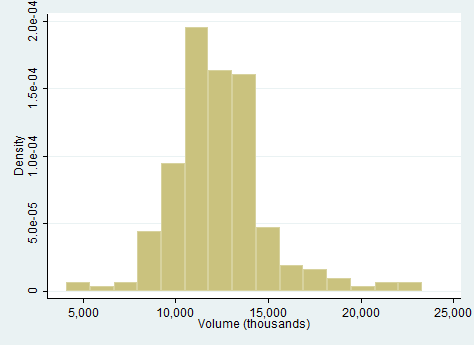
\includegraphics[height=4.1cm]{Graph.png}}
\end{column}
\begin{column}{5cm}
{\footnotesize 
\texttt{sysuse sp500}\\
\texttt{histogram volume, normal}}\\\medskip
\centerline{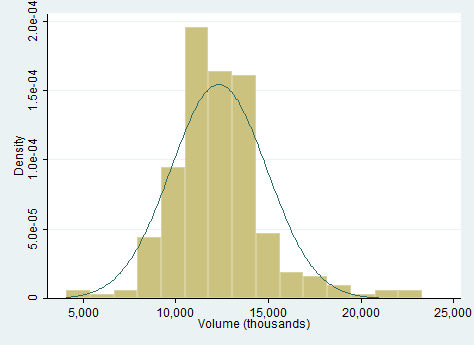
\includegraphics[height=4.1cm]{Graph1.png}}
\end{column}
\end{columns}
\end{frame}

 
\begin{frame}{Ejemplo histograma}{}
Para describir mejor los gráficos en general (no solo el histograma) tenermos las siguientes opciones:
\begin{itemize}
\item \texttt{title(\textit{nombre del gráfico})}
\item \texttt{subtitle(\textit{subtítulo del gráfico})}
\item \texttt{note(\textit{nota al final del gráfico})}
\item \texttt{caption(\textit{fuente del gráfico})}
\end{itemize}
Los ejes tienen como título por defecto al nombre de la variable. Para cambiarlo:
\begin{itemize}
\item \texttt{xtitle(\textit{título del eje x})}
\item \texttt{ytitle(\textit{título del eje y})}
\end{itemize}
\end{frame}

\begin{frame}{Ejemplo histograma}{}
{\footnotesize \texttt{histogram volumen, title(título) subtitle(subtítulo) /// note(NOTA) xtitle(ejex) ytitle(ejey) caption(fuente)}}\\\medskip
\centerline{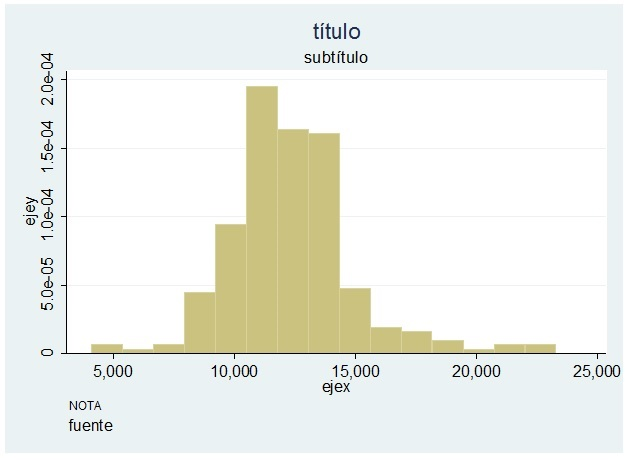
\includegraphics[height=5.5cm]{hist.jpg}}
\end{frame}

\section{twoway}
\subsection{Introducción}
\begin{frame}{Gráficos ``twoway''}
\begin{itemize}
\item Muestra la relación entre dos variabes numéricas.
\item \texttt{twoway} es el comando básico para los gráficos twoway, que pueden ser, entre otros, los siguientes \textit{plottypes}:
\begin{itemize}
\item \texttt{scatter} 
\item \texttt{line} 
\item \texttt{connected}  
\item \texttt{area} 
\item \texttt{bar} 
\item \texttt{dropline} 
\item \texttt{lfit} 
\item \texttt{spike} 
\end{itemize}
\item En los ejemplos utilizamos datos sobre la esperanza de vida en Estados Unidos para el periodo 1900-1940:\\
{\footnotesize \texttt{use http://www.stata-press.com/data/r12/uslifeexp2}}
\end{itemize}
\end{frame}

\begin{frame}{Gráficos ``twoway''}{Ejemplos}
\begin{columns}
\begin{column}{5cm}
{\footnotesize 
\texttt{twoway scatter le year}}\\\medskip
\centerline{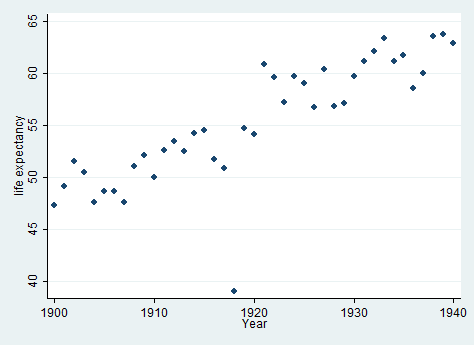
\includegraphics[height=4.1cm]{twscatter.png}}
\end{column}
\begin{column}{5cm}
{\footnotesize 
\texttt{twoway lfitci le year}}\\\medskip
\centerline{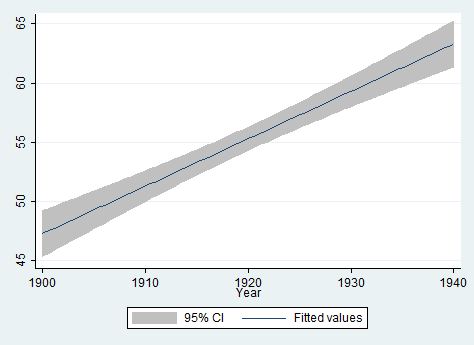
\includegraphics[height=4.1cm]{twlf.png}}
\end{column}
\end{columns}
\end{frame}


\begin{frame}{Gráficos ``twoway''}{Ejemplos}
\begin{columns}
\begin{column}{5cm}
{\footnotesize 
\texttt{twoway bar le year}}\\\medskip
\centerline{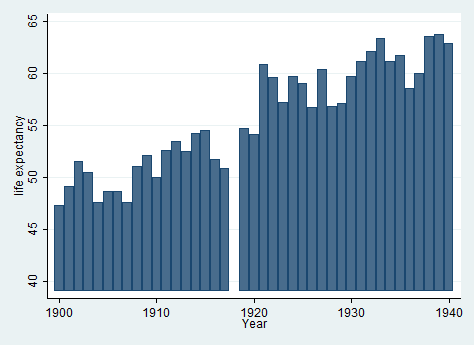
\includegraphics[height=4.1cm]{twbar.png}}
\end{column}
\begin{column}{5cm}
{\footnotesize 
\texttt{twoway connected le year}}\\\medskip
\centerline{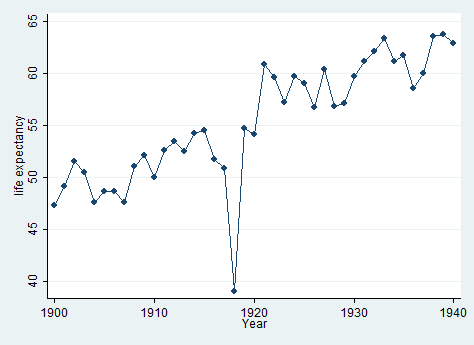
\includegraphics[height=4.1cm]{twcon.png}}
\end{column}
\end{columns}
\end{frame}

\begin{frame}{Gráficos ``twoway''}{Ejemplos}
{\footnotesize \texttt{twoway area le year, title(``Evolución de la esperanza de vida'') subtitle(``Estados Unidos, 1900-1940") xtitle(``año") ytitle(``") note(``National Vital Statistics Report")}}\\\medskip
\centerline{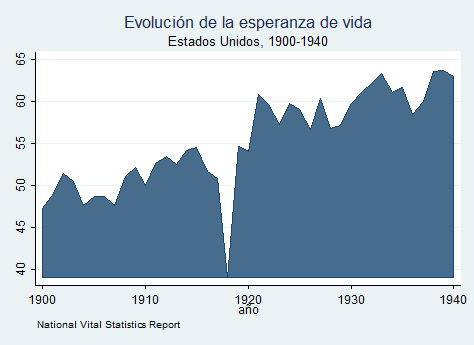
\includegraphics[height=4.2cm]{twarea.png}}
\end{frame}


\begin{frame}{Gráficos ``twoway''}{Opciones específicas}
\begin{itemize}
\item Si en la línea de comandos escribimos: \texttt{palette symbol} aparece el siguente gráfico\\\medskip
\centerline{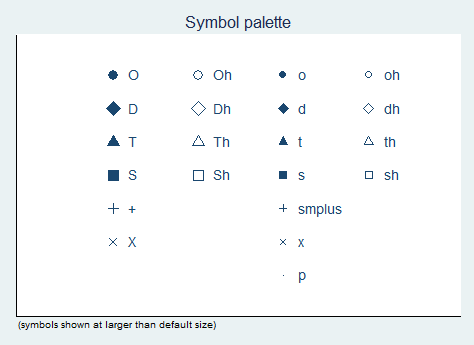
\includegraphics[height=4cm]{twop.png}}
\item Con la opción \texttt{msymbol()} podemos cambiar el símbolo.
\end{itemize}
\end{frame}

\begin{frame}{Gráficos ``twoway''}{Ejemplos}
{\footnotesize 
\texttt{twoway scatter le year, msymbol(th)}}\\\medskip
\centerline{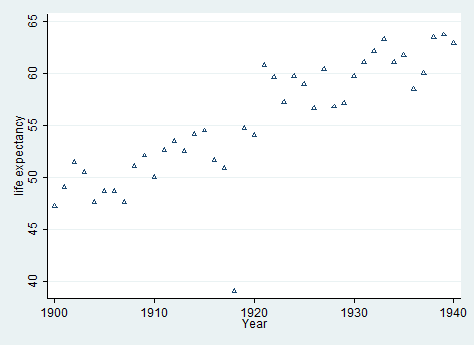
\includegraphics[height=5.1cm]{twscatter1.png}}
\end{frame}

\subsection{Superposición de gráficos}

\begin{frame}{Superponer gráficos}
\begin{itemize} 
\item Los gráficos se pueden superponer:\\
{\footnotesize \texttt{twoway (scatter  le year)  (lfit le year)}}\\\smallskip
\centerline{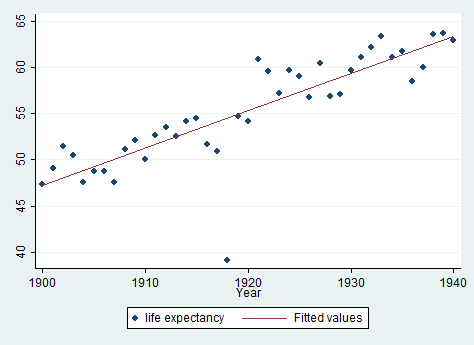
\includegraphics[height=3.8cm]{twsup.png}}
\item Las opciones a todo el gráfico van al final, después de una coma. Las opciones para cada uno de los gráficos individuales van al interior del paréntesis.
\end{itemize}
\end{frame}


\begin{frame}{Gráficos ``twoway''}{Ejemplos}
{\footnotesize \texttt{twoway (scatter le year, msymbol(th)) (lfit le year), title(``Evolución de la esperanza de vida'') subtitle(``Estados Unidos, 1900-1940") xtitle(``año") ytitle(``") note(``National Vital Statistics Report")}}\\\medskip
\centerline{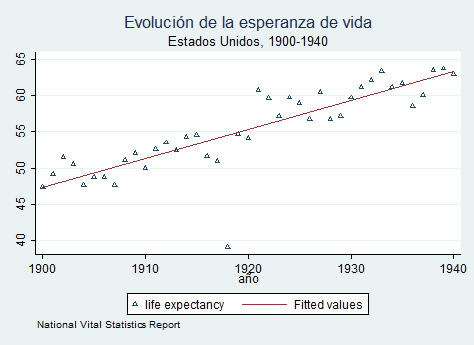
\includegraphics[height=4.1cm]{twsup1.png}}
\end{frame}

\subsection{uso del by()}
\begin{frame}{uso del by()}
\begin{itemize}
\item Los gráficos admiten la opción \texttt{by()}:
\end{itemize}
{\footnotesize \texttt{sysuse auto.dta, clear}}\\
{\footnotesize \texttt{twoway scatter mpg weight, by(foreign)}}\\\medskip
\centerline{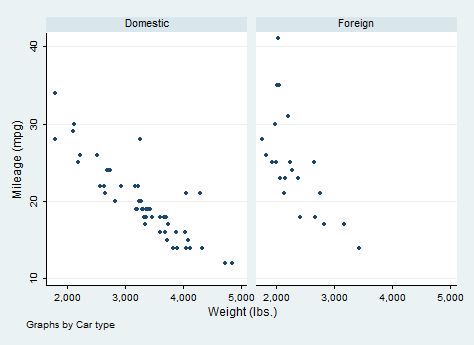
\includegraphics[height=4.1cm]{by.png}}
\end{frame}

\subsection{Combinar gráficos}

\begin{frame}{combinar gráficos}
\begin{itemize}
\item Podemos realizar distintos gráficos por separado e ir guardándolos con la opción \texttt{saving()}.
\item Luego los combinamos con el comando \texttt{graph combine}.
\end{itemize}
\centerline{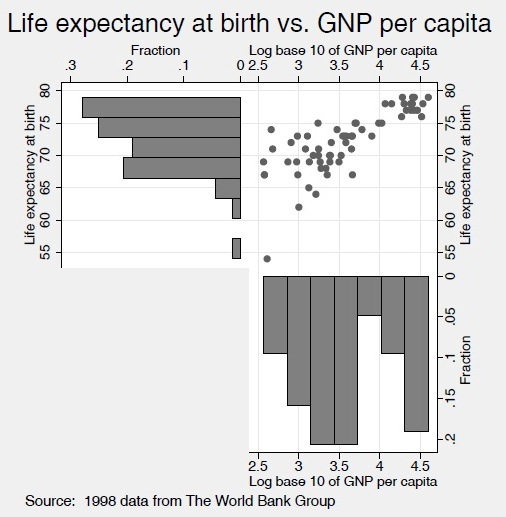
\includegraphics[height=5cm]{graf4.jpg}}
\end{frame}

\section{Gráficos de barras}

\begin{frame}{gráfico de barras}
\begin{itemize}
\item \texttt{graph bar} grafica barras verticales, donde en el eje $y$ se muestran estadísticos de variables numéricas y en el eje $x$, variable/s categórica/s.
\end{itemize}
{\footnotesize \texttt{sysuse citytemp}}\\
{\footnotesize \texttt{graph bar (mean) tempjuly tempjan, over(region)}}\\\medskip
\centerline{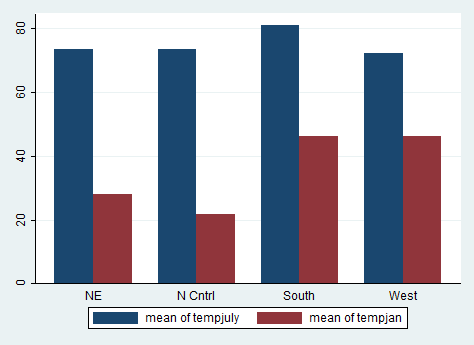
\includegraphics[height=3.4cm]{bar.png}}
\end{frame}

\begin{frame}{gráfico de barras}
\begin{itemize}
\item La opción \texttt{over} se puede repetir, mostrando categorías para más de una vairable.
\item La opción \texttt{nofill} hace que no se muestren las categorías missing.
\end{itemize}
{\footnotesize \texttt{graph hbar (mean) tempjan, over(division) over(region)}}\\\medskip
\centerline{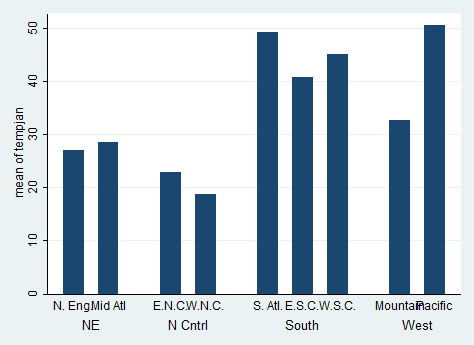
\includegraphics[height=4cm]{bar1.png}}
\end{frame}

\section{Box plots}
\begin{frame}{Box plots}
\begin{itemize}
\item \texttt{graph box} /\texttt{graph hbox} grafica la distribución de una variable numérica. La parte inferior de la caja es el p25 y la superior, el p75. También se indican \textit{outliers}.
\end{itemize}
{\footnotesize \texttt{sysuse nlsw88, clear}}\\
{\footnotesize \texttt{graph hbox wage, over(ind)}}\\\medskip
\centerline{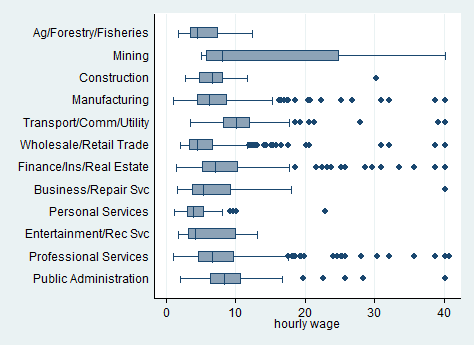
\includegraphics[height=3.8cm]{box.png}}
\end{frame}

\section{Line}

\begin{frame}{Líneas}
\begin{itemize}
\item Este tipo de gráfico se utiliza mucho en el caso de series de tiempo. Como ejemplo cargamos la base:
\end{itemize}
{\footnotesize \texttt{sysuse uslifeexp.dta}}\\
{\footnotesize \texttt{line le\_wfemale le\_wmale le\_wm le\_bm year}}\\\medskip
\centerline{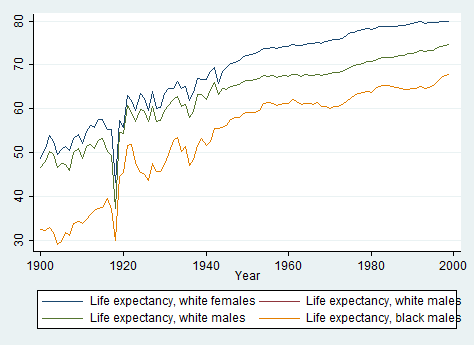
\includegraphics[height=4cm]{line.png}}
\end{frame}


\begin{frame}{Opciones}
\begin{itemize}
\item Si en la línea de comandos escribimos \texttt{palette linepalette} aparece el siguiente gráfico:\\\smallskip
\centerline{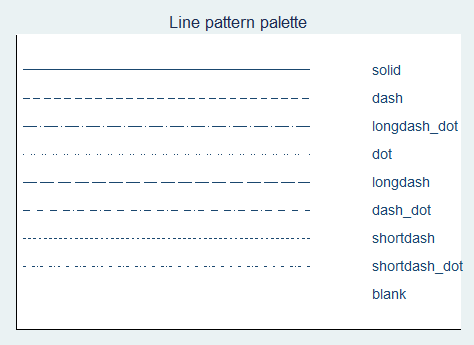
\includegraphics[height=3cm]{pale.png}}
\item Con la opción \texttt{lpattern()} podemos cambiar el patrón de la línea.
\item Similarmente, con las opciones \texttt{lcolor()} y \texttt{lwidth()} cambiamos el color y grosor de las líneas, respectivamente. 
\end{itemize}
\end{frame}

\begin{frame}{Opciones}{}
{\footnotesize \texttt{line le\_wfemale le\_wmale le\_wm le\_bm year, lpattern(solid dash dot longdash) lcolor(red blue black green) lwidth(thick thin thick thin)}}\\\medskip
\centerline{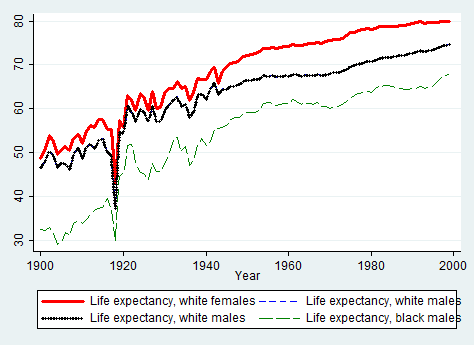
\includegraphics[height=4cm]{pale1.png}}
\end{frame}

\end{document}


Indicator values for levels of factor variables

Regresiones en STATA
Series de tiempo
graficos
macros, escalares y bucles

